\documentclass[12pt]{article}
\usepackage[utf8]{inputenc}
\usepackage{graphicx}
\usepackage{listings}
\usepackage{amsmath}
\usepackage{tensor}
\usepackage{subfigure}
\usepackage{float}
\usepackage{natbib}
\usepackage{url}
\usepackage{color}
\usepackage{hyperref}

%Include packages to have python(or other prog. languages) scripts included in the pdf-file without broken lines

\definecolor{codegreen}{rgb}{0,0.6,0}
\definecolor{codegray}{rgb}{0.5,0.5,0.5}
\definecolor{codepurple}{rgb}{0.58,0,0.82}
\definecolor{backcolour}{rgb}{0.95,0.95,0.92}
\lstdefinestyle{mystyle}{
    backgroundcolor=\color{backcolour},
    commentstyle=\color{codegreen},
    keywordstyle=\color{magenta},
    numberstyle=\tiny\color{codegray},
    stringstyle=\color{codepurple},
    basicstyle=\footnotesize,
    breakatwhitespace=false,
    breaklines=true,
    captionpos=b,
    keepspaces=true,
    numbers=left,
    numbersep=5pt,
    showspaces=false,
    showstringspaces=false,
    showtabs=false,
tabsize=2}
\lstset{style=mystyle}

%Making vectors bold instead of putting arrow on it
\renewcommand{\vec}[1]{\mathbf{#1}}

% Roman numbers
\newcommand{\RNum}[1]{\uppercase\expandafter{\romannumeral #1\relax}}


\begin{document}

\begin{titlepage}

\newcommand{\HRule}{\rule{\linewidth}{0.5mm}}
\center

\textsc{\LARGE University of Oslo}\\[1.5cm]
\textsc{\Large FYS4150}\\[0.5cm]
\textsc{\large Kristine Moseid, Helene Aune, \& Helle Bakke}\\[0.5cm]

\begin{minipage}{0.4\textwidth}
\end{minipage}\\[1cm]

\HRule \\[0.4cm]
{ \huge \bfseries Introduction to numerical projects}\\[0.4cm]
\HRule \\[1.5cm]

\begin{minipage}{0.4\textwidth}
\end{minipage}\\[8cm]

{\large \today}\\[3cm]
\vfill

\end{titlepage}

\newpage
\tableofcontents

\newpage



\begin{abstract}
\noindent We used Gaussian elimination to create algorithms for both a general and special case of a tridiagonal matrix. The results for each case were compared to each other with regards to floating point operations. The algorithms for the general case were compared to a closed-form solution, which showed us that large values of $n$ gives small relative errors. We used the C++ library \textit{'armadillo'} and solved the tridiagonal matrix with LU decomposition. When compared to the tridiagonal matrix method, the LU decomposition showed to be less CPU time efficient.
\end{abstract}



\section{Introduction}

\noindent The aim of this project is to solve the one-dimensional Poisson equation with Dirichlet boundary conditions by rewriting it as a set of linear equations. We will be solving the equation

\begin{align*}
    \frac{d^2\phi}{dr^r} = -4 \pi r \rho(r)
\end{align*}

\noindent By letting $\phi \rightarrow u$ and $r \rightarrow x$ it is simplified to

\begin{align*}
    -u^{\prime \prime}(x) = f(x), \quad x \in (0,1), \quad  u(0) = u(1) = 0
\end{align*}

\noindent where we define the discretized approximation to $u$ as $v_i$ with grid point $x_i = ih$ in the interval from $x_0$ to $x_{n+1} = 1$, and the step length as $h = 1/(n+1)$. \\

\noindent By doing this we will be able to create algorithms for solving the tridiagonal matrix problem, and find out how efficient this is compared to other matrix elimination methods.

\newpage

%%%%%% METHODS %%%%%%%%%%%%%%
\section{Methods}


%%%%%%%%% A %%%%%%%
\subsection{Tridiagonal matrix}

\noindent With the bounadry condition $v_0 = v_{n+1} = 0$, the approximation of the second derivative of $u$ was written as

\begin{align*}
    - \frac{v_{i+1} + v_{i-1} - 2v_i}{h^2} = f_i, \quad i = 1,...,n
    \intertext{where $f_i = f(x)$. We rewrote the equation as a linear set of equations:}
    - (v_{i+1} + v_{i-1} - 2v_i) = h^2f_i
    \intertext{We set $h^2f_i = d_i$, and solved this equation for a few values of $i$.}
    \intertext{$i = 1$:}
    - (v_{1+1} + v_{1-1} - 2v_1) &= d_1 \\
    - (v_2 + v_0 - 2v_1) &= d_1 \\
    - v_2 - 0 + 2v_1 &= d_1
    \intertext{$i = 2$:}
    - (v_{2+1} + v_{2-1} - 2v_2) &= d_2 \\
    - v_3 - v_1 + 2v_2) &= d_2
    \intertext{$i = 3$:}
    - (v_{3+1} + v_{3-1} - 2v_3) &= d_3 \\
    - v_4 - v_2 + 2v_3) &= d_3
\end{align*}
\begin{align*}
    \intertext{We saw that this could be written as a linear set of equations $\vec{A} \vec{v} = \vec{d}$,}
    \begin{bmatrix}
     	2  & -1 & 0  & \dots & \dots & 0 \\
        -1 &  2 & -1 & 0     & \dots & \dots \\
        0  & -1 & 2  & -1    & 0     & \dots \\
           & \dots   & \dots & \dots & \dots & \dots \\
        0  & \dots   &       & -1    & 2     & -1 \\
        0  & \dots   &       & 0     & -1    & 2 \\
    \end{bmatrix}
    \begin{bmatrix}
    	v_1 \\
    	v_2 \\
    	v_3 \\
    	\dots \\
    	v_{n-1} \\
    	v_n \\
    \end{bmatrix}
	=
    \begin{bmatrix}
    	d_1 \\
    	d_2 \\
    	d_3 \\
    	\dots \\
    	d_{n-1} \\
    	d_n \\
	\end{bmatrix}
\end{align*}

%%%% END A %%%%%%%


%%%%%%%%%%%%%%  B  %%%%%%%%%%%%%%%%%%%%%%%%%

\subsection{Forward substitution}

The following tridiagonal matrix was written in a general form. For simplicity, we made a $4 \times 4$ matrix with rownumbers of  \( \vec{A} \) in red. \\
\begin{align*}
    \begin{matrix}
        \textcolor{red}{I} \\
        \textcolor{red}{II} \\
        \textcolor{red}{III} \\
        \textcolor{red}{IV}
    \end{matrix}
    \begin{bmatrix}
        {b_1} & {c_1} & 0     & 0    \\
        0     & {b_2} & {c_2} & 0     \\
        0     & 0     & {b_3} & {c_3}  \\
        0     & 0     & 0     & {b_4}   \\
    \end{bmatrix}
    \begin{bmatrix}
        v_1 \\
        v_2 \\
        v_3 \\
        v_4
    \end{bmatrix}
    =
    \begin{bmatrix}
        d_1 \\
        d_2 \\
	    d_3 \\
        d_4 \\
    \end{bmatrix}
\end{align*}
\\
\noindent We used a simplified form of Gaussian elimination, known as the tridiagonal matrix algorithm \citep{WikiT} to solve the above system. First, we decomposed $\vec{A}$ and used forward substitution so that $a_2$, $a_3$ and $a_4$ equaled to zero. We gave the decomposed rows the new name $\tilde{b_i}$.\\

\noindent Since row $\RNum{1}$ did not have any $a$'s to remove, we moved on to the next row. We got:

\begin{align*}
    \widetilde{\RNum{2}} = \RNum{2} - \RNum{1}  k_1 = (0, \ \tilde{b_2}, \ c_2, \ 0)     \\
    k_1 = \frac{a_2}{b_1}, \ \ \ \tilde{b_2} = b_2 - \frac{a_2 c_1}{b_1} \\
    \widetilde{\RNum{3}} = \RNum{3} - \widetilde{\RNum{2}}  k_2 = (0, \ 0 \ \tilde{b_3}, \ c_3) \\
    k_2 = \frac{a_3}{\tilde{b_2}}, \ \ \ \tilde{b_3} = b_3 - \frac{a_3 c_2}{\tilde{b_2}}\\
\end{align*}

\noindent After doing this for a couple more rows we clearly saw that the algorithm for $k_i$ and $\tilde{b_i}$ could be generalized to:

\begin{align*}
    k_i = \frac{a_{i+1}}{b_i}, \qquad \tilde{b_i} = b_i - \frac{a_i c_{i-1}}{\tilde{b_i}} \\
\end{align*}

\noindent Our newly forward substituted (and simplified) matrix now looked like this:

\begin{align*}
    \begin{matrix}
        \textcolor{red}{I} \\
        \textcolor{red}{\widetilde{II}} \\
        \textcolor{red}{\widetilde{III}} \\
        \textcolor{red}{\widetilde{IV}}
    \end{matrix}
    \begin{bmatrix}
        {b_1} & {c_1}        & 0           & 0        \\
        0     & \tilde{b_2}  & {c_2}       & 0     \\
        0     & 0            & \tilde{b_3} & {c_3}  \\
        0     & 0            & 0           & \tilde{b_4}  \\
    \end{bmatrix}
    \begin{bmatrix}
        v_1 \\
        v_2 \\
        v_3 \\
        v_4
    \end{bmatrix}
    =
    \begin{bmatrix}
        d_1 \\
        \tilde{d_2} \\
        \tilde{d_3} \\
        \tilde{d_4} \\
    \end{bmatrix}
\end{align*}

%\clearpage
\subsection{Backward substitution}

\noindent We wrote these matrices out as linear equations and solved them for $v_i$ to find the backward substitution algorithm, starting with the last row:

\begin{align*}
    \RNum{4}: \tilde{b_4}v_4 = \tilde{d_4} \\
    \RNum{3}: \tilde{b_3}v_3 + c_3 v_4 = \tilde{d_3} \\
    \RNum{2}: \tilde{b_2}v_2 + c_2 v_3 = \tilde{d_2} \\
    \Rightarrow v_i = \frac{\tilde{d_i} - c_i v_{i+1}}{\tilde{b_i}}\\
\end{align*}

\noindent Finally, our backward substitution gave us the correct algorithm for $\tilde{d_i}$,

\begin{align*}
    \tilde{d_2} &= \widetilde{\RNum{2}} \bf{v} = (\RNum{2} - \RNum{1}  k_1) \bf{v} = \RNum{2} \bf{v} - \RNum{1} k_1 \bf{v} = d_2 - d_1 k_1 \\
    \tilde{d_3} &= \widetilde{\RNum{3}} \bf{v} = (\RNum{3} - \RNum{2}  k_2) \bf{v} = \RNum{3} \bf{v} - \RNum{2} k_2 \bf{v} = d_3 - d_2 k_2 \\
    \Rightarrow \tilde{d_i} &= d_i - d_{i-1} k_{i-1}
\end{align*}

\noindent We had found the algortihms for solving the tridiagonal matrix problem, and we implemented them into a C++ script.
%%%%%%%% END B%%%%%%%%%%%


%%% C %%%%
\subsection{Tridiagonal matrix algorithm for special case}

Now we wanted to specialize our algorithm to the special case where the matrix had identical elements along the diagonal, and identical values for the diagonal elements. To make it easy to solve analytically we used a $4 \times 4$-matrix and decomposed it, before we used Gaussian elimination to create a forward and backward substitution algorithm like the above.

\bigskip
\noindent Decomposition:

\begin{align*}
    \begin{matrix}
        \textcolor{red}{I} \\
        \textcolor{red}{II} \\
        \textcolor{red}{III} \\
        \textcolor{red}{IV}
    \end{matrix}
    \begin{bmatrix}
        2  & -1 & 0  & 0 \\
        -1 & 2  & -1 & 0 \\
        0  & -1 & 2  & -1 \\
        0  & 0  & -1 & 2
    \end{bmatrix}
    \begin{bmatrix}
        v_1 \\
        v_2 \\
        v_3 \\
        v_4
    \end{bmatrix}
    =
    \begin{bmatrix}
        d_1 \\
        d_2 \\
        d_3 \\
        d_4
    \end{bmatrix}
\end{align*}

\noindent Forward substitution:

\begin{align*}
    \widetilde{\RNum{2}} = II - I \cdot \left( - \frac{1}{2} \right) &= \left( 0, \frac{3}{2}, -1, 0 \right)\\
    \widetilde{\RNum{3}} = III - \widetilde{\RNum{2}} \cdot \left( - \frac{2}{3} \right) &= \left( 0, 0, \frac{4}{3}, -1 \right) \\
    \widetilde{\RNum{4}} = IV - \widetilde{\RNum{3}} \cdot \left( - \frac{3}{4} \right) &= \left(0, 0, 0, \frac{5}{4} \right) \\
    \intertext{From this, we found algorithms for \( \tilde{b}_{\text{spec, i}} \) and $k_i$: } \smallskip
    \tilde{b}_{\text{spec, i}} = \frac{i+1}{i}, \quad \quad k_i &= - \frac{i}{i+1}
    \\
    \intertext{Backward substitution:}
    \begin{bmatrix}
        2 & -1                      &                         & 0 \\
          & \tilde{b}_{\text{spec}, 2} & -1 \\
        0 &                         & \tilde{b}_{\text{spec}, 3} & -1 \\
          &                         &                         & \tilde{b}_{\text{spec}, 4}
    \end{bmatrix}
    \begin{bmatrix}
        v_1 \\
        v_2 \\
        v_3 \\
        v_4
    \end{bmatrix}
    &=
    \begin{bmatrix}
        d_1 \\
        \tilde{d}_2 \\
        \tilde{d}_3 \\
        \tilde{d}_4
    \end{bmatrix}
\end{align*}

\begin{align*}
    \tilde{b}_{\text{spec}, 4} \cdot v_4 = \tilde{d}_4 \quad &\Rightarrow \quad v_4 = \frac{\tilde{d}_4}{\tilde{b}_{\text{spec}, 4}}  \\
    \tilde{b}_{\text{spec}, 3} \cdot v_3 - v_4 = \tilde{d}_3 \quad &\Rightarrow \quad v_3 = \frac{\tilde{d}_3 + v_4}{\tilde{b}_{\text{spec}, 3}} \\
    \intertext{We found a general algorithm for this special case:}
    v_i = \tilde{d}_{i+1} &+ \frac{\tilde{d}_i}{\tilde{b}_{\text{spec}, i}}
\end{align*}

\noindent The specialized algotihms were implemented in a new C++ script.
%%%%% END C %%%%%%%

\newpage

%%%%% D %%%%%%
\subsection{Relative error}
\noindent We computed the relative error in the data set $i = 1,...,n$ by using the expression

\begin{align*}
    \epsilon_i = log_{10} \Big( \Big| \frac{v_i - u_i}{u_i}  \Big| \Big),
\end{align*}

\noindent using $v_i$ from the general backward substitution algorithm. We implemented the closed-form solution $u(x) = 1 - (1 - e^{-10})x - e^{-10x}$ to our code and calculated the relative error when increasing $n$ to $n = 10^7$.
%%%%% END D %%%%%%%


%%%%% E
\subsection{LU decomposition}

\noindent Lastly, we wanted to use the C++ library \textit{'armadillo'} to solve the LU decomposition for matrices of size $10 \times 10$, $100 \times 100$ and $1000 \times 1000$. We implemented the linear equation $$\vec{A} = \vec{L} \vec{u}$$ and used

\begin{lstlisting}
    // find the LU decomposition
    lu(L,U,A);
\end{lstlisting}

\noindent to solve it.\\

\noindent We also tried to run the code for a matrix of size $10^5 \times 10^5$, to see if our computer could handle such a large matrix.
%%%%% END 



%%%%%%%%% RESULTS %%%%%%%%%%%%%
\section{Results}

%%%%%% B %%%%%%%%%%%

\subsection{Tridiagonal matrix algorithm vs. closed form soultion}

\noindent We used Python to plot the general algorithm for three different values of $n$ with the closed-form solution $u(x)$.

\begin{figure}[H]
    \centerline{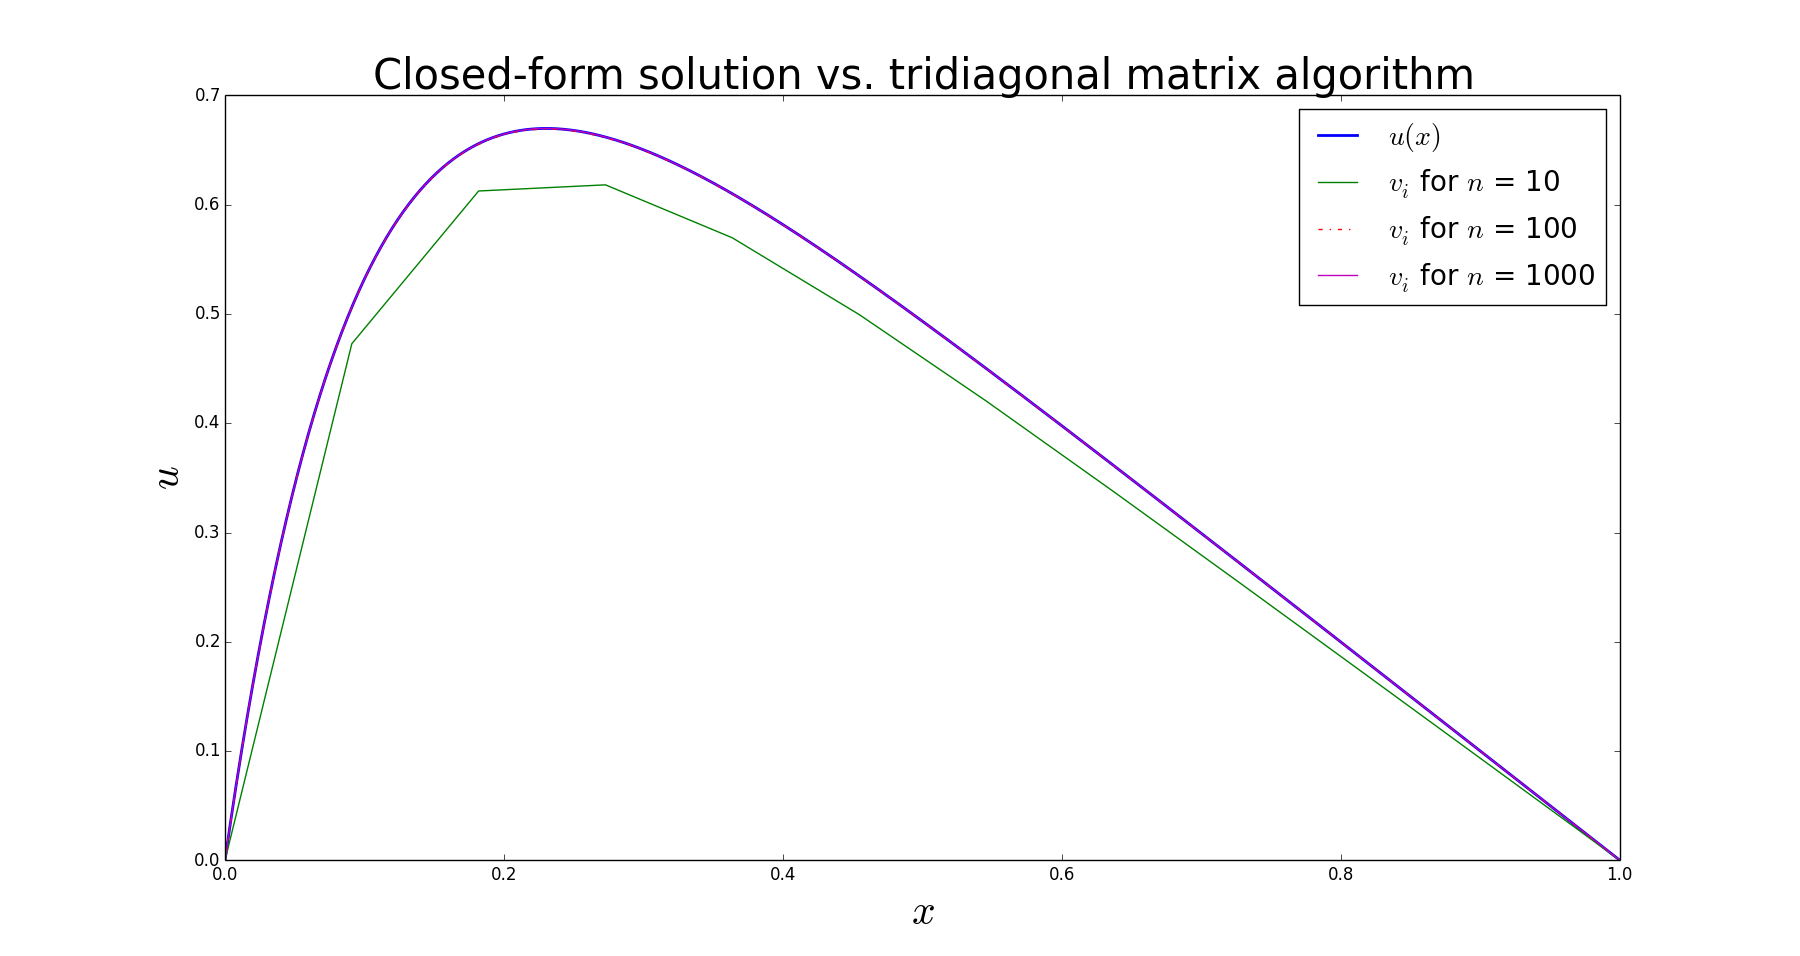
\includegraphics[width=1.3\textwidth]{figure_1b.png}}
    \caption{Closed form solution(blue) versus the tridiagonal matrix algorithm for $n = 10$     (green), $n = 100$ (red lines), and $n = 1000$ (pink line). }
    \label{fig:1b}
\end{figure}

\begin{figure}[H]
    \centerline{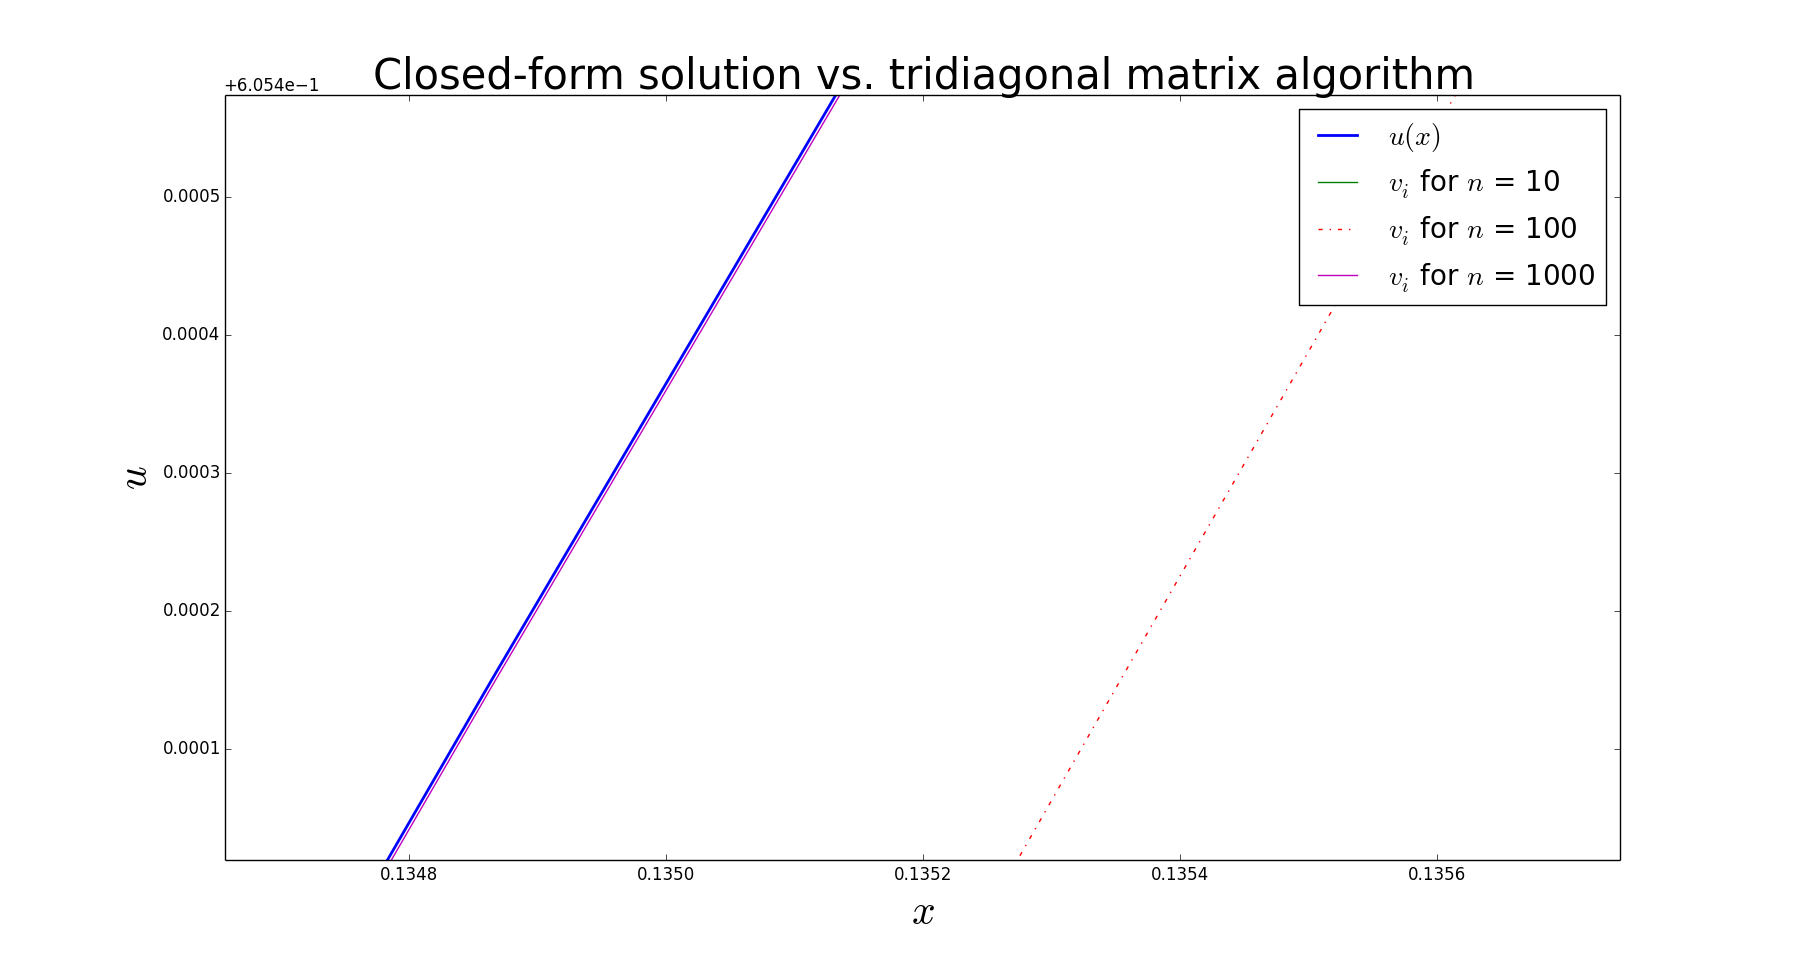
\includegraphics[width=1.3\textwidth]{figure_1b_zoom.png}}
    \caption{Figure \ref{fig:1b} zoomed.}
    \label{fig:1bz}
\end{figure}

\noindent Figure \ref{fig:1b} shows how the general tridiagonal matrix algorithm for three different $n$'s compare to the closed-form solution. We saw that for $n = 10$ (green) we got, as expected, the biggest difference.\\

\noindent The latter three curves were harder to distinguish, so Figure \ref{fig:1bz} shows a zoomed version of Figure \ref{fig:1b}. We saw that the larger $n$-values gave a better approximation to the closed-form solution, were $n = 1000$ aligned almost perfectly with $u(x)$\\ 

%%%% END B %%%%%

\subsection{Floating point operations}

\noindent FLOPS is an acronym for \textit{floating point operations per second} \citep{WikiF}, and is an useful tool to measure computer perfomance. \\

\noindent Table \ref{tab:fl1} shows the variable names from our general algorithm with their corresponding floating point operation. $\tilde{b_i}$ was a special case, as the relation $\frac{c_{i-1}}{b_{i-1}}$ only needed to be computed once. Therefore, the amount of FLOPS was 3 the first time $\tilde{b_i}$ was calculated, then 2. \\

\begin{table}[H]
    \centering
    \begin{tabular}{ l | c }
        &FLOPS \\ \hline
        $\tilde{b_i}$ & 2 (3) \\
        $k_i$& 1 \\
        $v_i$ & 3 \\
        $\tilde{d_i}$ & 2 \\
    \end{tabular}
    \caption{Floating point operations for the tridiagonal matrix}
    \label{tab:fl1}
\end{table}

\noindent The total number of floating point operations for the tridiagonal matrix was then computed to be $8n$, and $9n$ the first time the algorithms were calculated.

%%%%% C  %%%%%%


\subsection{Tridiagonal algorithm for special case}

\noindent We created a table with the CPU time for the general and special algorithms:

\begin{table}[H]
    \centering
    \begin{tabular}{ c | c | c }
    	$n$ & CPU time general & CPU time special \\
    	\hline
    	10     & 4e-6     & 3e-6 \\
    	$10^2$ & 8e-6     & 5e-6 \\
    	$10^3$ & 6.7e-5   & 2.3e-5 \\
    	$10^4$ & 6.08e-4  & 4.4e-4 \\
    	$10^5$ & 0.004186 & 0.002676 \\
    	$10^6$ & 0.037559 & 0.024366 \\
    \end{tabular}
    \caption{CPU time for general and special algorithm}
    \label{tab:cpu}
\end{table}
\medskip

\noindent We saw that the special algortihm was a bit faster than the general. We also counted a total of $8n$ floating point operations for the special algorithm. \\

%%%%% END C %%%%%%%%%



%%%% D %%%%%%%%
\subsection{Relative error}

\noindent In our Python code we took the minimum value of each list of error values. This was because the error values became negative, as a result of $u(x)$ being exponential. We created a table of the relative error results:

\begin{table}[H]
    \centering
    \begin{tabular}{ c | c }
    	$n$ & $\epsilon$ \\
    	\hline
    	10 & -1.1797 \\
    	$10^2$ & -3.08804 \\
    	$10^3$ & -5.08005 \\
    	$10^4$ & -7.07936 \\
    	$10^5$ & -9.0049 \\
    	$10^6$ & -6.77137 \\
    	$10^7$ & -12.8074\\
    \end{tabular}
	\caption{Table of the relative error $\epsilon$ for increasing $n$}
    \label{tab:err}
\end{table}
\medskip

\noindent Table \ref{tab:err} shows the relative error $\epsilon$ for increasing $n$. We saw that the error became smaller when $n$ increased, but for $n = 10^6$ this was not the case. Since the function was exponential, we suggested that it might have had something to do with loss of precision in the process. 
%%%%%%% END D %%%%%%%



%%%%%%  E  %%%%%%%%%
\subsection{LU decomposition}

\noindent We created a table of the calculated CPU time for both the tridiagonal matrix and the LU decomposition:

\begin{table}[H]
    \centering
    \begin{tabular}{ l | c | r }
        n & Tridiagonal method & LU method \\ \hline
        10 & 4.0e-6 & 3.0e-5 \\
        100 & 7.0e-6 & 1.0e-3 \\
        1000 & 5.7e-5& 8.8e-2 \\
    \end{tabular}
    \caption{CPU time of tridiagonal matrix and LU decomposition}
    \label{tab:LU}
\end{table}

\noindent From Table \ref{tab:LU} we saw that the general algorithm for a tridiagonal matrix was faster in CPU time than that of a LU decomposition. \\

\noindent The number of floating point operations for the LU decomposition is $\frac{2}{3}n^3$\citep{LU}. We noticed that the program used some time to execute the command, and the matrix of size $10^5 \times 10^5$ did not execute at all. This was because the memory needed to create the matrix was too big for our computer. We calculated how much memory was needed to create the matrix:

\begin{align*}
    \frac{10^5 \cdot 10^5 \cdot 64}{8} &= \frac{8 \cdot 10^{10}}{1024} \enskip \text{B} \\
    &= \frac{78125000}{1024} \enskip \text{kB} \\
    &= \frac{762939}{1024} \enskip \text{MB} \\
    &= 74.5 \enskip \text{GB}
\end{align*}

\noindent It was with good reason that our computer where not able to execute the program for this matrix size.

 %%%%%% END E %%%%%



\section{Conclusion}

\noindent Although it may be tempting to use \textit{'armadillo'} to solve matrix decompositions, our results showed that it was more efficient to create algorithms to solve the tridiagonal matrix problem. The CPU time for forward and backward substitution was shorter than for the LU decomposition. The relative error when solving the algorithms became smaller for larger values of $n$. However, the figures showed us that we did not need very large values of $n$ to get a good approximation to the exact function. Calculating the algorithms for large vectors took a longer time, and we learned that we did not have to do this to get a good result. \\

\noindent As an improvement, we could have worked more with our programs. We calculated, analytically, that the tridiagonal matrix algorithms used $8n$ floating point operations, but in our code we implemented this so that it always used $9n$ floating point operations. Therefore, Table \ref{tab:cpu} showed a little difference in CPU time for the general and special algorithms.  



\section{Appendix}

\noindent To run the programs, one needs to give an input argument. This argument varies between $1,...,7$, and refers to the exponent of $10$ for each $n$-value. This applies to the programs \textit{'project1\_main.cpp'} and \textit{'project1\_c.cpp'}. \\

\noindent The program \textit{'project1\_main.cpp'} contains the algorithms calculated in exercise 1b, the calculation of the relative error $\epsilon_i$ in exercise 1d and the calculation of CPU time. The program \textit{'project1\_c.cpp'} contains the specialized algorithm, and the QT folder contains the LU decomposition using the \textit{'armadillo'} library. \\

\noindent The program \textit{'project1\_python.py'} contains the plotting of figures in exercise 1b, as well as a calculation of the maximum value in each error list. All text-files are created in the main C++ program, and imported into the Python program for further computations. \\

\noindent The programs can be found on he GitHub address \url{https://github.com/hellmb/CompPhys/tree/master/Project%201}


\addcontentsline{toc}{section}{References}
\nocite{*}
\bibliographystyle{plain}
\bibliography{project1}


\end{document}
